\section{Multi-way tables}\label{sec:ca-multiway}

A three- or higher-way table can be analyzed by correspondence
analysis in several ways.
\ixon{correspondence analysis!stacking}
Multiple correspondence analysis (MCA), described in \secref{sec:mca},
is an extension of simple
\CA\ which analyzes simultaneously all possible two-way tables
contained within a \mway\ table.
Another approach, described here, is called 
\glossterm{stacking}.
\ix{interactive coding}
A
three-way table, of size \(I \times  J \times  K\) can be sliced into
\(I\) two-way tables, each \(J \times  K\).  If the slices are
concatenated vertically, the result is one two-way table, of size \((
I \times  J ) \times  K\).  In effect, the first two variables are
treated as a single composite variable with \(IJ\) levels, which represents the main
effects and interaction between the original variables that were
combined.
\Citet{HeijdenLeeuw:85}
discuss this use of
correspondence analysis for multi-way tables and show how \emph{each} way of
slicing and stacking a contingency table corresponds to the analysis
of a specified \loglin\ model.
Like the mosaic display, this provides another way to visualize the relations
in a \loglin\ model.

In particular, for the three-way table that is reshaped as a table of
size \(( I \times  J ) \times  K\), the \CA\
solution analyzes residuals from the log-linear model [AB] [C].  That
is, for such a table, the \(I \times  J\) rows represent the joint
combinations of variables A and B.  The expected frequencies under
independence for this table are
\begin{equation}\label{eq:mij-k}
  m_{[ij]k} = \frac{ n_{[ij]+} \,  n_{[+]k} }{n}
 = \frac{ n_{ij+} \,  n_{++k} }{n}
\end{equation}
which are the ML estimates of expected frequencies for the log-linear
model [AB] [C].  The \(\chi^2\) that is decomposed by \CA\ is the Pearson
\(\chi^2\) for this log-linear model.  When the table is stacked as
\(I \times  ( J \times  K )\) or \(J \times  ( I \times  K )\),
correspondence analysis decomposes the residuals from the log-linear
models [A] [BC] and [B] [AC], respectively.
\Citet{HeijdenLeeuw:85}
show how a generalized form of correspondence analysis
can be interpreted as decomposing the difference between two specific
log-linear models, so their approach is more general than is illustrated
here.

This approach to the \CA\ of \mway\ tables is easily carried out with the
\proc{CORRESP} and the \macro{CORRESP}.  With the procedure, use the
\stmt{TABLES}{CORRESP} and list the variables to be combined interactively
as either the row or column variables (separated by a comma).
For example,  the \CA\ of residuals from the model [A B][C] of joint independence
\eqref{eq:mij-k} is specified by:

\begin{listing}
proc corresp cross=row;
   tables A B, C;
   weight count;
\end{listing}
The \opt{CROSS}{CORRESP} specifies that all combinations of the levels
of A and B are to define the rows of the \ctab.%
\footnote{If this option is omitted, the separate levels of each of
A and B define the table rows.}

For the \macro{CORRESP}, the
list the variables
in the \mparm{TABLES=}{CORRESP} separated by a \texttt{/},%
\footnote{You can also use a comma, but then the \mparm{TABLES=}{CORRESP}
must be quoted with the \pname{\%str()} macro function, e.g.,
\pname{TABLES=\%str(A B, C)}.}
and include \pname{CROSS=BOTH|ROW|COL} in the \mparm{OPTIONS=}{CORRESP}.
The following statement is equivalent to that above:
\begin{listing}
%corresp(options=cross=row,
   tables=A B/ C, weight=count);
\end{listing}

\begin{Example}[suicide1]{Suicide rates in Germany}

To illustrate the use of correspondence analysis for the analysis for
three-way tables, we use data on suicide rates in West Germany
(presented in \tabref{tab:suidat})
classified by age, sex, and method of suicide used.  The data, from
\citet[Table 1]{Heuer:79}
have been discussed by
\citet{Friendly:91,Friendly:94a,HeijdenLeeuw:85}
and others.
The original \(2
\times  17 \times  9\) table contains 17 age groups from 10 to 90 in
5-year steps and 9 categories of suicide method, listed in \datref{dat:suicide}. 
To avoid extremely
small cell counts and cluttered displays,
this example uses a reduced table in which age
groups are combined in 15 year intervals except for the last
interval, which includes age 70 - 90; the methods ``toxic gas'' and
``cooking gas'' were collapsed and methods ``knife'' and ``other''
were deleted, giving the \(2 \times  5 \times  6\) table shown in
\tabref{tab:suidat}.  These changes do not affect the general
nature of the data or conclusions drawn from them.

\input{ch5/tab/suidat}
\tabref{tab:suifit} shows the results of all possible hierarchical
log-linear models for the suicide data.  It is apparent that none of
these models has an acceptable fit to the data.  Given the enormous
sample size (\(n = 48,177\)), even relatively small departures from
expected frequencies under any model would appear significant,
however.
\begin{table}[htb]
 \caption{Goodness-of-fit for hierarchical
log-linear models for the suicide data}\label{tab:suifit}
 \begin{center}
 \begin{tabular}{lrrrrr}
 \hline
  Model & df & L.R. \(G^2\) & G.F. \(\chi^2\) \\ 
   \hline
  $[M] [A] [S]$ & 49 & 10119.60 & 9908.24 \\ [2mm]
%
  $[M] [AS]$ & 45 & 8632.0 & 8371.3 \\ 
  $[A] [MS]$ & 44 & 4719.0 & 4387.7 \\ 
  $[S] [MA]$ & 29 & 7029.2 & 6485.5 \\ [2mm]
%
  $[MS] [AS]$ & 40 & 3231.5 & 3030.5 \\ 
  $[MA] [AS]$ & 25 & 5541.6 & 5135.0 \\ 
  $[MA] [MS]$ & 24 & 1628.6 & 1592.4 \\ [2mm]
%
  $[MA] [MS] [AS]$ & 20 & 242.0 & 237.0 \\ 
 \hline
 \end{tabular}
 \end{center}
\end{table}


The decision about which variables to combine interactively relates
more to the choice of which associations are to be displayed,
and which are to be ignored, rather than to the choice of a best-fitting
model.  For example,
\CA\ applied to the [AS] by [M] table helps to
show the nature of the association between method of suicide and the
joint age-sex combinations and decomposes the \(\chi^2 = 8371\) for
the log-linear model [AS] [M].  This analysis would ignore the
age-sex association, however.

To carry out this analysis with the
data in the form of a frequency \Dset\
(with variables \texttt{age}, \texttt{sex}, \texttt{method}, and
\texttt{count}),
call the \proc{CORRESP} with the statements
\begin{listing}
proc corresp data=suicide cross=row short;
   table age sex, method;
   weight count;
run;
\end{listing}
Or, to perform this analysis and produce the graphical display in
\figref{fig:suicide51}, call the \macro{CORRESP} as
\begin{listing}
axis1 order=(-.7 to .7 by .7) length=6.5 in label=(a=90 r=0);
axis2 order=(-.7 to .7 by .7) length=6.5 in;
%corresp(data=suicide, tables=%str(age sex, method), weight=count,
        options=cross=row short, vaxis=axis1, haxis=axis2);
\end{listing}

\begin{figure}[htb]
  \centering
  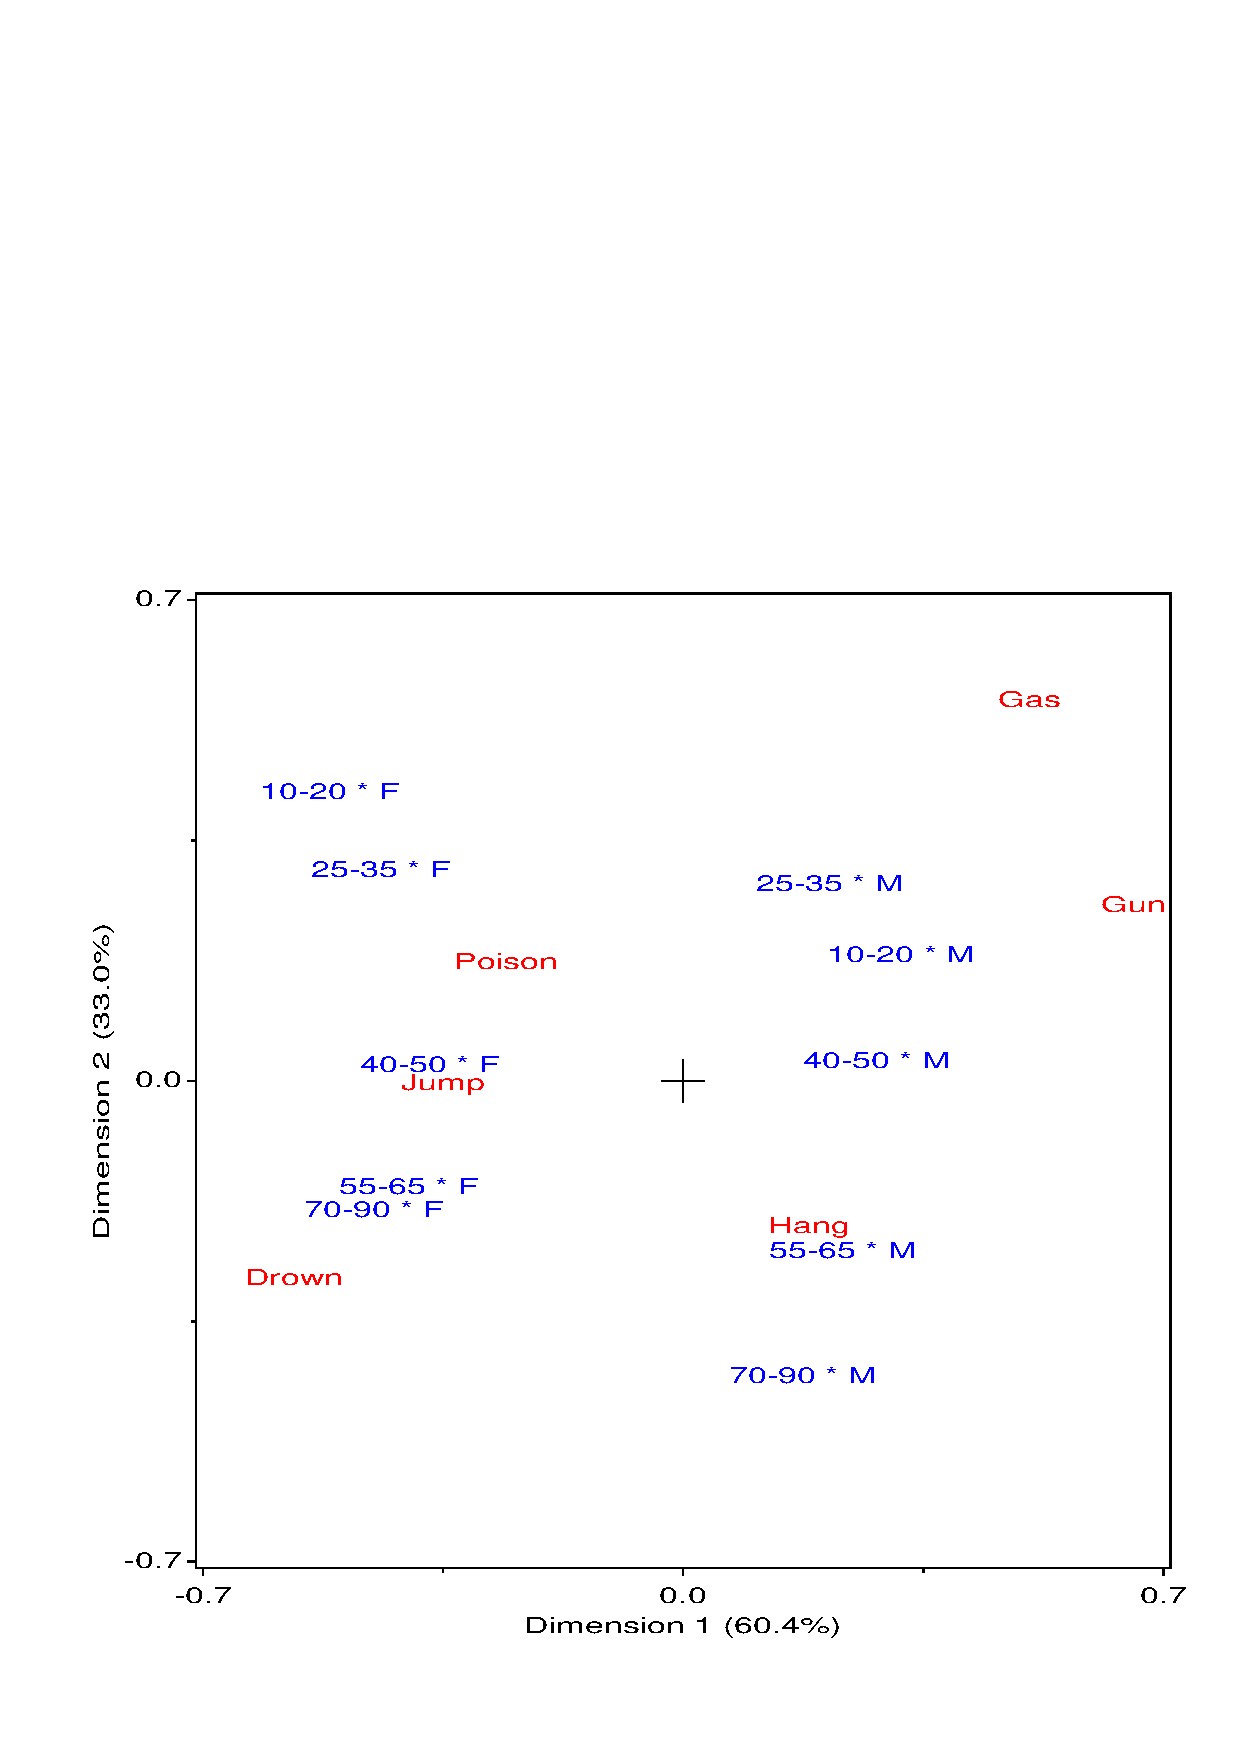
\includegraphics[scale=.7,clip=true]{ch\thechapter/fig/suicide51}
  \caption{Two-dimensional correspondence analysis
solution for the [AS] [M] multiple table}\label{fig:suicide51}
\end{figure}

The printed results, shown partially in \outref{out:suicide5} indicate that over 93\% of the association between the age-sex categories and method of
suicide can be represented well in two dimensions.

\begin{Output}[htb]
\caption{Chi-Square Decomposition for suicide data}\label{out:suicide5}
\begin{output}
                   Inertia and Chi-Square Decomposition

     Singular  Principal Chi-
     Values    Inertias  Squares Percents   12   24   36   48   60
                                         ----+----+----+----+----+---
     0.32138   0.10328   5056.91  60.41% *************************
     0.23736   0.05634   2758.41  32.95% **************
     0.09378   0.00879    430.55   5.14% **
     0.04171   0.00174     85.17   1.02%
     0.02867   0.00082     40.24   0.48%
               -------   -------
               0.17098   8371.28 (Degrees of Freedom = 45)
\end{output}
\end{Output}
\ixd{suicide}

The plot of the \CA\ scores for the rows (sex-age combinations) and
columns (methods) in \figref{fig:suicide51}
shows residuals from the log-linear model [AS] [M].
Thus, it shows the two-way associations of sex \(\times\) method, age
\(\times\) method, and the three-way association, sex \(\times\) age
\(\times\) method which are set to zero in the model [AS] [M].  The
possible association between sex and age is not shown in this plot.

Dimension 1 in the plot separates males and females.  This dimension
indicates a strong difference between suicide profiles of males and
females.  The second dimension is mostly ordered by age with younger
groups at the top and older groups at the bottom.  Note also that the
positions of the age groups are approximately parallel for the two
sexes.  Such a pattern indicates that sex and age do not interact in
this analysis.  The relation between the age - sex groups and methods
of suicide can be interpreted in terms of similar distance and
direction from the origin, which represents the marginal row and
column profiles.  Young males are more likely to commit suicide by
gas or a gun, older males by hanging, while young females are more
likely to ingest some toxic agent and older females by jumping or
drowning.

For comparison, the mosaic display for the [AS] [M] table
is shown in \figref{fig:mosaic6b}.
The methods have been arranged in order
of the method scores on the first dimension of the CA solution
of \figref{fig:suicide51}.
This figure
again shows the prevalence of GUN and
GAS, among younger males and decreasing with age, whereas use of HANG
increases with age.  For females, these three methods are used less
frequently than would be the case if method were independent of age
and sex, whereas POISON, JUMP, and DROWN occur more often.

\begin{figure}[!htb]
  \centering
  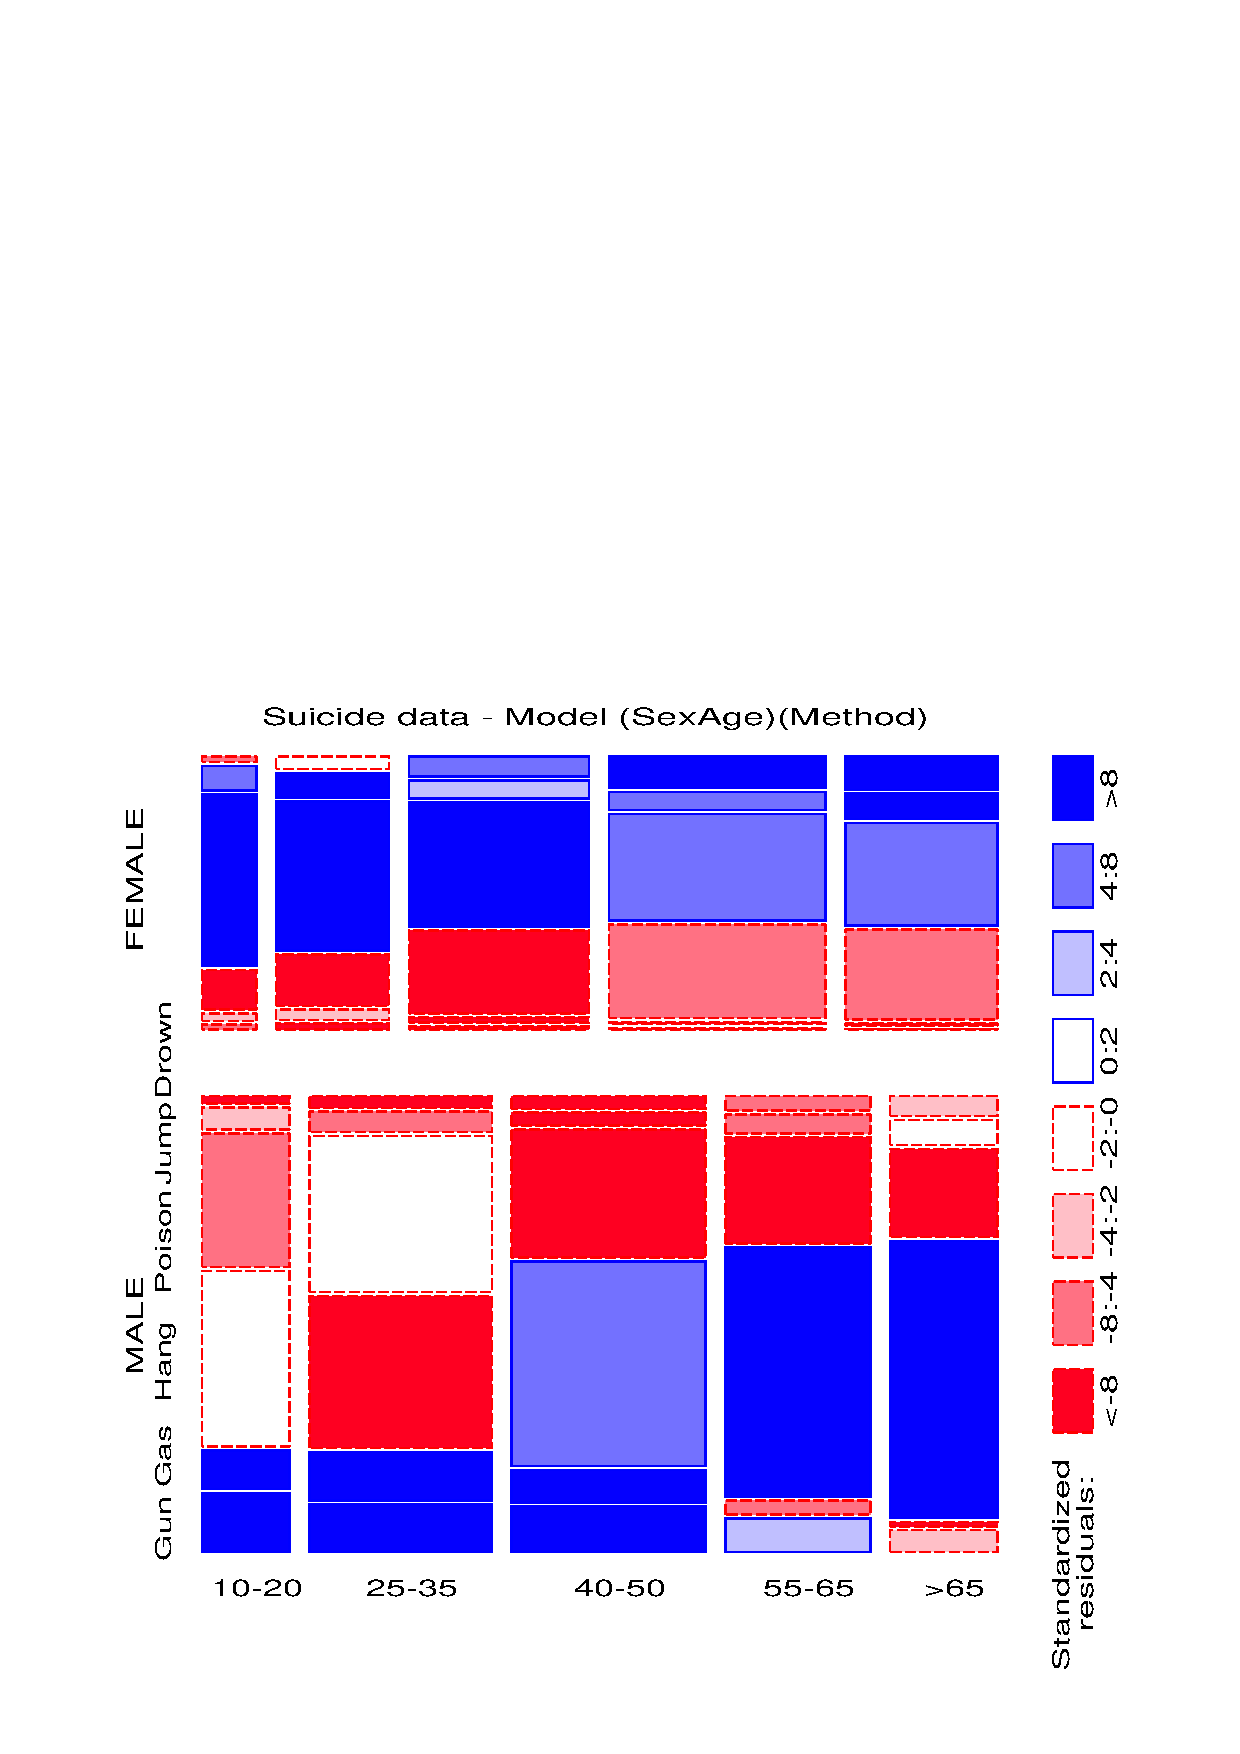
\includegraphics[scale=.6,clip]{ch\thechapter/fig/mosaic6b}
  \caption[Mosaic display showing deviations from
model AS, M]{Mosaic display showing deviations from
model [AS] [M].  The methods have been reordered according to their
positions on Dimension 1 of the correspondence analysis solution for
the [AS] [M] table.}\label{fig:mosaic6b}
\end{figure}
\end{Example}
\ixoff{correspondence analysis!stacking}

\subsection{Marginal tables and supplementary variables}
\ix{correspondence analysis!supplementary variables}
An \nway\ table in frequency form or case form is automatically collapsed
over factors which are not listed in the
\stmt{TABLES}{CORRESP} (or in the macro \mparm{TABLES=}{CORRESP}).
The analysis gives a marginal model for the categorical variables which
\emph{are} listed.  

The positions of the categories of the omitted variables
may nevertheless be recovered, by treating them as supplementary variables.
A supplementary variable is ignored in finding the CA solution,
but its categories are then projected into that space.

To illustrate, the statement below lists only the \texttt{age}
and \texttt{method} variables, and hence produces an analysis
collapsed over \texttt{sex}.
This ignores not only the effect of sex itself,
but also all associations of age and method with sex,
which (from \tabref{tab:suifit}) are substantial.
\begin{listing}
%corresp(data=suicide, tables=%str(age, method),  weight=count);
\end{listing}

This analysis and 
the graph produced do not include category points for \texttt{sex},
but we may re-do the same analysis including \texttt{sex} as a supplementary
variable as shown below.

\begin{listing}
%corresp(data=suicide, tables=%str(age sex, method), sup=sex,
   weight=count, inc=0.2 0.1, dimlab=Dim);
\end{listing}
Note that \texttt{sex} must also be listed among the \pname{TABLES}
variables.
\begin{figure}[htb]
  \centering
  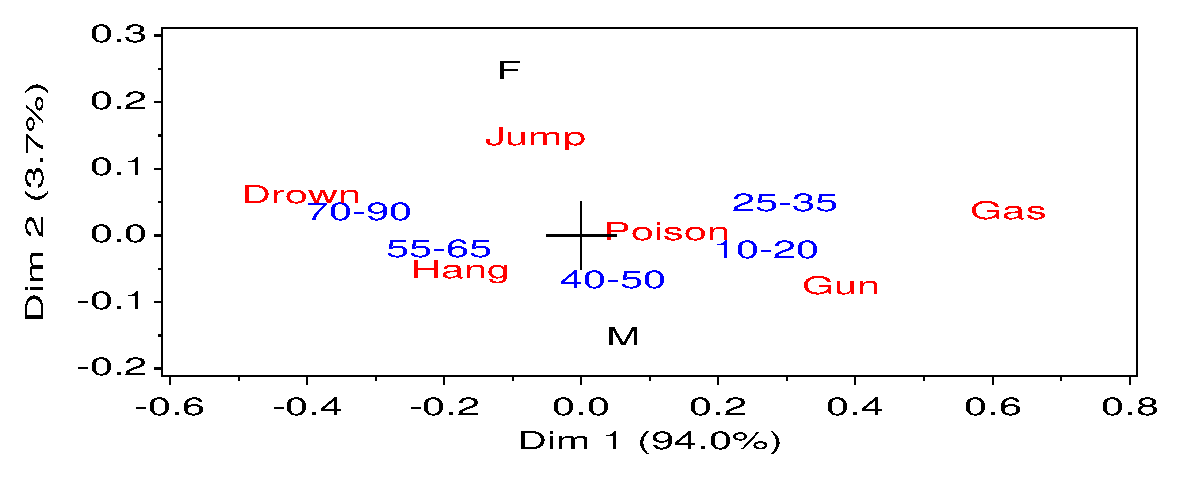
\includegraphics[scale=.7,clip=true]{ch\thechapter/fig/suicide6}
  \caption[Two-dimensional correspondence analysis
solution for the A M marginal table]{Two-dimensional correspondence analysis
solution for the [A] [M] marginal table.
Category points for Sex are shown as supplementary points.}\label{fig:suicide6}
\end{figure}

This analysis produces a $\chisq (20) = 2917.83$,
the same as the Pearson chi-square for the [A] [M] marginal table.
The plot (\figref{fig:suicide6}) is essentially one-dimensional,
where Dimension 1 reflects age most prominently.
Comparing this graph with \figref{fig:suicide51},
you may see that ignoring sex has collapsed the differences between
males and females which were the dominant feature of the analysis
including sex.
However, as in \figref{fig:suicide51}, the supplementary points for sex 
show a greater tendency for females to use JUMP, and for males to use
HANG or GUN.
